\documentclass[twocolumn,aps]{revtex4}
\usepackage[utf8]{inputenc}
\usepackage[T1]{fontenc}
\usepackage{lmodern}
\usepackage[ngerman]{babel}
\usepackage{graphicx}
\graphicspath{{./img/}}
\begin{document}
\title{Kräfte im hängenden Seil}
\author{Gert-Ludwig Ingold}
\affiliation{Institut für Physik, Universität Augsburg, 86135 Augsburg}
\begin{abstract}
  In diesen Notizen soll die maximale Kraft hergeleitet werden, die in einem
  undehnbaren hängenden Seil auftritt. Dazu wird zunächst mit Hilfe der 
  Betrachtung der auf ein kurzes Seilstück wirkenden Kräfte der Seilverlauf,
  die sogenannte Kettenlinie, hergeleitet. Anschließend lässt sich die maximale
  Seilkraft bestimmen.
\end{abstract}
\maketitle

\section{Herleitung der Kettenlinie}
Zunächst wird der Seilverlauf eines undehnbaren, im Gravitationsfeld hängenden
Seils, die sogenannte Kettenlinie, berechnet. Es handelt sich dabei um ein
Variationsproblem mit Nebenbedingungen, in dem die potentielle Energie des
Seils bei vorgegebener Seillänge $L$ minimiert werden soll. Dies kann mit 
Hilfe von Lagrange-Multiplikatoren und der zugehörigen Euler-Lagrange-Gleichung
erfolgen. Da wir uns aber in erster Linie für die Seilkräfte interessieren,
ist es angebracht, die Kettenlinie stattdessen durch eine Kräftebetrachtung
herzuleiten.

\begin{figure}
 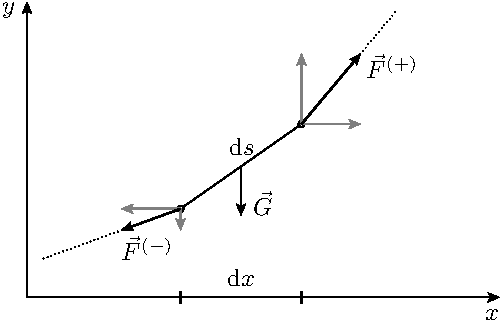
\includegraphics[width=0.8\columnwidth]{kraefte}
 \caption{Auf ein kurzes Seilstück der Länge $\mathrm{d}s$ wirken
	  die Gewichtskraft $\vec G$ sowie die Seilkräfte $\vec F^{(-)}$
	  und $\vec F^{(+)}$ von links bzw.\ von rechts. Die grau
	  dargestellten Vektoren zerlegen die Seilkräfte in die
	  horizontalen und vertikalen Komponenten.}
\end{figure}
\end{document}
